\begin{figure}[h][p]
    \centering
    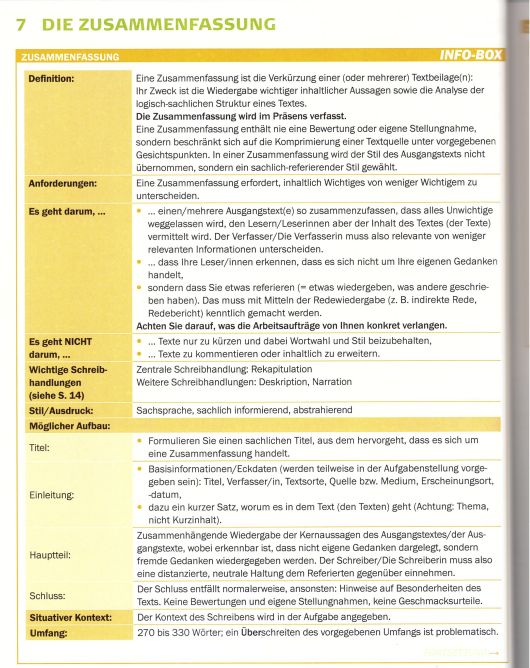
\includegraphics[scale=0.8]{./pics/Screenshot from 2023-02-06 12-32-33.png}
    \caption{Zusammenfassung: Definition + Aufbau}
    \label{fig:impl:Zusammenfassung1}
\end{figure}
\begin{figure}[h]
    \centering
    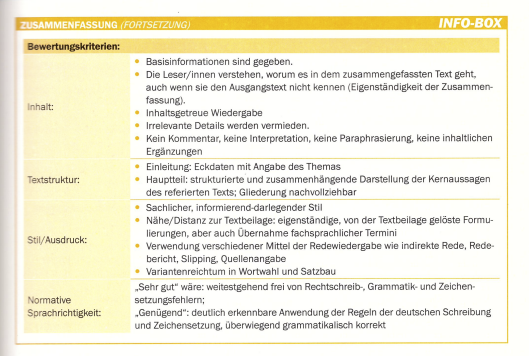
\includegraphics[scale=0.8]{./pics/Screenshot from 2023-02-06 12-33-05.png}
    \caption{Zusammenfassung: Verfassen}
    \label{fig:impl:Zusammenfassung2}
\end{figure}
\begin{figure}[h]
    \centering
    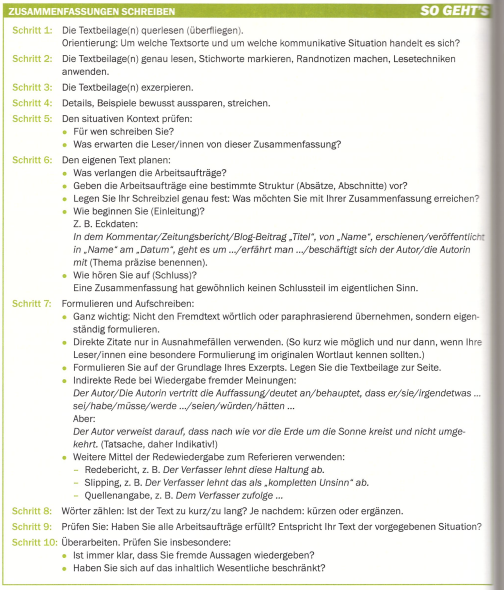
\includegraphics[scale=0.8]{./pics/Screenshot from 2023-02-06 12-33-47.png}
    \caption{Zusammenfassung: Fortsetzung}
    \label{fig:impl:Zusammenfassung3}
\end{figure}
  

\section{Mustertext}

Musterlösung 

In dem Drama "Faust. Der Tragödie erster Teil” von Johann Wolfgang von Goethe, veröffentlicht 1808 in der Weimarer Klassik, geht es um Doktor Heinrich Faust, der sich dem Teufel verschreibt, um seine Begierde nach Erkenntnis zu stillen. 

Der Wissenschaftler steckt in einer Krise und sucht Antworten, die er durch seine Forschung jedoch nicht finden kann. Er beschwört einen Erdgeist, doch dieser macht sich nur lustig über ihn. Von seiner Unwissenheit geplagt, spielt er mit dem Gedanken, sich umzubringen. 

 

Am nächsten Tag macht Faust mit seinem Assistenten Wagner einen Spaziergang, bei dem diese von einem schwarzen Hund verfolgt werden, den Faust schließlich mit zu sich nach Hause nimmt. Dort offenbart sich der Hund als Mephisto, der Teufel. Dieser unterbreitet Faust ein Angebot: Der Teufel verspricht ihm Erkenntnis, wenn dieser ihm dafür seine Seele gibt. 

 

Daraufhin will Mephisto Faust zeigen, wie schön das Leben sein kann. Sie gehen in eine Kneipe und Mephisto bringt Faust anschließend zu einer Hexe. Sie verabreicht ihm einen Zaubertrank, der ihn für Frauen begehrenswert macht. Faust erblickt das Abbild einer attraktiven Frau in einem Zauberspiegel. Danach gehen Mephisto und er in die Stadt, wo sie auf Gretchen treffen, die der Frau aus dem Zauberspiegel zum Verwechseln ähnlich sieht. 

 

Faust möchte Gretchen unbedingt für sich gewinnen. Mephisto nähert sich währenddessen Gretchens Nachbarin an, indem er den Tod ihres verschollenen Mannes beteuert. Gretchen und Faust können nun alleine sein und es kommt zum Kuss. Gretchen verliebt sich ebenfalls in Faust. Ihm wird aber zunehmend bewusst, dass er das Mädchen durch den Pakt mit seinem Teufel in ihr Unheil treiben könnte. 

 

Faust kann Gretchen überzeugen der Mutter ein Schlafmittel zu verabreichen, so dass die beiden die Nacht ungestört verbringen können. Das Mittel erweist sich jedoch als tödlich. Als Folge der gemeinsamen Nacht ist Gretchen schwanger, was ihr Bruder Valentin mitbekommt und Faust zur Rede stellt. Es kommt zum Kampf, bei dem Valentin stirbt. 

Mephisto reist daraufhin mit Faust zur Walpurgisnacht, bei der ausgelassene Stimmung herrscht. Er will Faust ablenken, doch dieser kann nur an Gretchen denken und erfährt schließlich, dass sie hingerichtet werden soll, weil sie ihr Neugeborenes aus Verzweiflung ertränkte. Faust kommt um Gretchen zu retten, doch diese will nicht mitgehen, da sie Mephisto als Teufel erkennt. Gretchen stirbt, gelangt aber durch Gott in den Himmel und wird von ihren Sünden erlöst. Faust schafft es, vor Mephisto zu fliehen. 

 

Quelle: \href{https://www.schreiben.net/artikel/dos-und-donts-dein-weg-zur-perfekten-zusammenfassung-665/ }{https://www.schreiben.net/artikel/dos-und-donts-dein-weg-zur-perfekten-zusammenfassung-665/ }



\section{Eigener Text}
\subsection{Angabe}
Lesen Sie den Zeitungsbericht „Die junge Generation ist benachteiligt“, der von Wolfgang Böhm verfasst wurde und in Die Presse am 13. November 2016 veröffentlicht wurde. Schreiben Sie nun eine Zusammenfassung und bearbeiten Sie folgende Arbeitsaufträge: Geben Sie die wichtigsten Inhalte hinsichtlich Jugendarbeitslosigkeit wieder. Beschreiben Sie die Vorzüge, die sich für die ältere Generation ergeben. Erschließen Sie die notwendigen Schritte, um einen sozialen Kollaps zu vermeiden.  

Schreiben Sie zwischen 270 und 330 Wörter. Markieren Sie Absätze mittels Leerzeilen 

\subsubsection{Die junge Generation ist benachteiligt}

Seit Beginn der Krise hat sich die soziale Kluft zwischen Jung und Alt vergrößert – und
das in ganz Europa. Der Anteil von Kindern und Jugendlichen ohne Zukunftschancen
steigt.

Gütersloh/Wien. Kinder und Jugendliche haben heute in der EU geringere Chancen auf einen
Job, ein gutes Gehalt und auf sozialen Aufstieg als frühere Generationen. Vor allem aber
verzeichnen sie ein höheres Armutsrisiko. Durch die Finanz- und Schuldenkrise hat sich ihre
Situation noch einmal verschlechtert. Während sich laut einer der „Presse“ exklusiv
vorliegenden Studie der Bertelsmann-Stiftung zur Entwicklung der sozialen Gerechtigkeit die
Lage der EU-Bürger in den Jahren nach der Krise insgesamt leicht verbessert hat, sind die
düsteren Zeiten für große Teile der Jugend nicht vorbei. Als „besonders bedenklich“ bewerten
die Studienautoren, dass sich die Kluft zwischen den Generationen durch die Krise ab 2008
vergrößert hat. „Die Älteren haben es geschafft, in der Krise ihre Sicherheit zu bewahren, die
Jugend nicht“, so Bertelsmann-Experte Daniel Schraad-Tischler.

Während der Anteil der von Armut und sozialer Exklusion (Ausgrenzung) bedrohten Kinder
und Jugendlichen in der EU seit 2008 von 26,4 auf nun 26,9 gestiegen ist, hat sich die Situation
der älteren Menschen wieder verbessert. Bei den über 65-Jährigen ist der Anteil der von Armut
bedrohten Menschen im selben Zeitraum von 23,3 Prozent auf 17,4 Prozent zurückgegangen.
Betroffen sind Personen, die erhebliche materielle Entbehrungen erleiden bzw. in einem
Haushalt mit sehr geringer Erwerbsbeteiligung leben.


Fast jeder zehnte Jugendliche in der EU (9,5\%) ist derzeit mit schwerwiegenden Entbehrungen
konfrontiert. Diese Personengruppe kann die Grundbedürfnisse des täglichen Lebens wie
Heizen oder Telefon nicht mehr decken. Bei den Älteren (über 65-Jährigen) liegt dieser Anteil
auf deutlich geringerem Niveau (5,5\%).
Ob Jobs, Gehalt oder Lebensumstände: Die ältere Generation sitzt wieder sicherer im Sattel,
während die Jugend den Einstieg in den Beruf und den Aufbau ihrer materiellen Existenz immer
schlechter bewältigt. Derzeit liegt die Jugendarbeitslosigkeit im EU-Schnitt bei 20,4 Prozent.
In den meisten europäischen Ländern wurden während der Krise die Einkommen älterer
Arbeitnehmer kaum gekürzt. Pensionszahlungen sind nicht oder nur geringfügig reduziert
worden. Die Einkommen der Jugend gingen im Gegensatz dazu zurück. Viele von ihnen
müssen zudem in Zukunft mit schlechteren Arbeitsverträgen leben als ihre Vorgänger.


Sozialer Zusammenhalt bedroht

Laut der Studie ist die soziale Teilhabe (Indikator aus Jobchancen, Bildungszugang,
Schulabbrecherquote, Armutsgefahr, Neet-Rate) der Jugend heute in keinem einzigen EU-Land
besser als im Jahr 2008. Österreich ist keine Ausnahme. Waren 2007 hier 16,7 Prozent der
Kinder und Jugendlichen (bis zu 18 Jahren) von Armut oder sozialer Exklusion bedroht, so sind 

es heute 18,3 Prozent. Bei der Generation der über 65-Jährigen ging dieses Risiko von 21,2 auf
14 Prozent zurück.
Es besteht ein deutliches Nord-Süd-Gefälle: Jugendliche aus Nordeuropa haben noch eher
Chancen auf einen Arbeitsplatz und ein geringeres Armutsrisiko als jene aus Südeuropa.
Besonders deutlich wird dieses Gefälle bei der sogenannten Neet-Rate. Sie fasst jenen Anteil
der Bevölkerung zusammen, der sich weder in einer beruflichen Ausbildung befindet noch einer
bezahlten Beschäftigung nachgeht. Im EU-Schnitt fallen 17,3 Prozent der 20- bis 24-Jährigen
in diese Kategorie. In Spanien liegt der Anteil bei 22 Prozent, in Italien sogar bei 31,1 Prozent.


Die Bertelsmann-Experten weisen zudem darauf hin, dass die steigende Verschuldung der EUStaaten ebenfalls zulasten der Jugend gehen dürfte. Denn sie muss künftig einen höheren Anteil
ihrer Gehälter für die Rückzahlung von Staatsschulden aufwenden als ihre Eltern und
gleichzeitig mit weniger sozialer Absicherung auskommen. Laut Aart de Geus, dem
Vorstandsvorsitzenden der Bertelsmann-Stiftung, bedroht diese Situation den
gesellschaftlichen Zusammenhalt. „Die wachsende Perspektivlosigkeit vieler junger Menschen
spielt den erstarkenden populistischen Bewegungen in die Hände.“

Um einer solchen Entwicklung entgegenzuwirken, fordern die Studienautoren Reformen in der
Arbeitsmarkt- und Bildungspolitik. Wichtig sei unter anderem ein gerechterer Zugang zu
Bildung. Denn derzeit gebe es einen starken negativen Einfluss des „sozioökonomischen
Hintergrunds“ auf den Lernerfolg der Jugendlichen. Kinder aus ärmeren Familien haben
deutlich geringere Chancen, ein höheres Bildungsniveau zu erreichen, als Kinder wohlhabender
Eltern. Länder wie Finnland oder Estland seien hier vorbildlich. Ihr Bildungssystem ermögliche
einen sozialen Durchstieg. Besonders schlecht steht es hingegen in Ungarn, der Slowakei,
Frankreich und Bulgarien.


\subsection{Text}
\subsubsection{Die junge Generation ist benachteiligt!}
Der Artikel „Die junge Generation ist benachteiligt“ von Wolfgang Böhm (Die Presse), welcher am 13.11.2016 erschienen ist, handelt von den Auswirkungen der Finanzkriese 2007. Vor allem der große Unterschied zwischen den Jugendlichen und Menschen über 65 wurde stark herausgehoben.  

Konkret geht es darum, dass vor allem die Älteren es geschafft haben, eine gewisse Sicherheit zu wahren, während bei den Jungen die Unsicherheit und die Angst der Zukunft wuchs. In Zahlen ausgedrückt heißt es, dass während der Krise die Zahl der Arbeitslosen Jugendlichen bei 26.4 \% lag, sie danach bei 26.9\%. Im Vergleich, bei den über 65-Jährigen schrumpfte der Anteil von 23.3\% auf 17.4 Prozent. Auch in den Zahlen der schwerwiegenden Entbehrungen spiegelt sich die Situation wider. Während 9.5\% der Jugendlichen in Europa ihre Grundbedürfnisse nicht decken können, sind es bei den Älteren lediglich 5.5 Prozent. Auslöser dafür war während der Krise die Tatsache, dass sich die Gehälter und Pensionen älterer Arbeitnehmer kaum gekürzt wurden, jedoch das Einkommen der Jungen stark zurück ging.   

Laut der Studie ist die soziale der Jugend heute in keinem einzigen EU-Landbesser als im Jahr 2008. Österreich ist keine Ausnahme. Waren 2007 hier 16,7 Prozent der Kinder und Jugendlichen (bis zu 18 Jahren) von Armut oder sozialer Exklusion bedroht, so sind es heute 18,3 Prozent. Bei der Generation der über 65-Jährigen ging dieses Risiko von 21,2 auf 14 Prozent zurück. Auch besonders bemerkenswert ist das deutliche Nord-Süd-Gefälle. Jugendliche aus Nordeuropa haben noch eher Chancen auf einen Arbeitsplatz und ein geringeres Armutsrisiko als jene aus Südeuropa.  

Am Ende des Artikels wird zu Arbeitsmarkt und Bildungspolitik Reformen aufgerufen, da sich die Lage der Jugendlichen zu verschlechtern scheint. Kinder aus ärmeren Familien haben deutlich geringere Chancen, ein höheres Bildungsniveau zu erreichen als Kinder wohlhabender Eltern. Länder wie Finnland oder Estland seien hier vorbildlich. 

\newpage


\section{Formulierungshilfen}

Einleitung:
enthält: Autor, Titel, Textsorte, Erscheinungsjahr/-datum, ggf. Erscheinungsort, kurze Benennung des Themas 
\begin{compactitem}
    \item Das/ Der /Die (Textsorte) „(Titel)“ von (Autor) aus dem Jahr .... beschreibt .../handelt von.../ thematisiert...  
    \item In dem (Zeitungsartikel) „(Titel)“ von (Autor) erschienen in (Erscheinungsort/ Herausgeber) am (Erscheinungsdatum) geht es um... 
\end{compactitem}
Hauptteil: 
\begin{compactitem}
    \item  Zu Beginn berichtet der Autor.../ spielt die Handlung... 
    \item  Anfangs wird festgestellt... / darauf hingewiesen, dass...
    \item  Eingangs .../ Zunächst.../ Bevor...
    \item Die Kurzgeschichte/ Der Roman/ Das Drama beginnt damit, dass... 
    \item Später geht der Autor darauf ein, dass... 
    \item  Im Folgenden... / Es folgt...
    \item Danach... / Später wird klar, dass...
    \item Im Verlauf der Geschichte/ des Berichtes/ des Kommentars etc. wird deutlich, dass...
    \item Plötzlich greift... in das Geschehen ein und.../ indem...
    \item  Die Situation beginnt sich zu verändern, als .../ nachdem... 
    \item Die Geschichte endet mit...
    \item Die Situation wird aufgelöst durch.../, indem.../ als..
    \item Schließlich .../ Am Ende.../ Zum Schluss... 
    \item Abschließend betont der Autor (nochmals), dass 
\end{compactitem}

Schluss:
\begin{compactitem}
    \item  Auf mich wirkt der Text... 
    \item  Zusammenfassend ist also pointiert festzuhalten, dass… 
    \item Letztlich bleibt anzumerken... 
    \item Als einzig logisches Fazit lässt sich also festhalten, dass...
    \item Abschließend ist daher anzunehmen, dass... 
    \item m Vergleich zu... ist es in diesem Text/ diesem Autor (nicht) gelungen... 
\end{compactitem}

\subsection{Erklärung}

Eine Zusammenfassung ist eine Textform, die einen längeren Text oder eine längere Informationsquelle auf dessen wesentliche Inhalte reduziert. Sie soll die wichtigsten Informationen des ursprünglichen Textes in verkürzter Form wiedergeben, ohne die wichtigsten Details zu verändern.

Eine gute Zusammenfassung sollte verständlich und aussagekräftig sein, ohne dass der Leser den Originalen Text kennen muss. Um eine Zusammenfassung zu schreiben, ist es wichtig, den ursprünglichen Text gründlich zu lesen und zu verstehen, um dann die wichtigsten Inhalte herauszufiltern und verständlich wiederzugeben.

Zusammenfassungen können in verschiedenen Kontexten verwendet werden, z.B. in Schulen oder Universitäten, um eine schnelle Übersicht über längere Texte oder Studienmaterialien zu erhalten.
\subsection{Realitätsbezug}
Die Zusammenfassung findet man oft im echten Leben. Sei es einfach, wenn man das gelesene wiedergeben möchte, oder für einen Test einfach den Stoff zusammenschreibt. Es ist meiner meinung einer der wichtigste, jedoch auch einer der einfachsten Textsorten, da man kaum eigenen Inhalt erschaffen muss, sondern einfach vorhandenen Inhalt logisch kürzen muss. 

\subsubsection{Beispiele für verwandte Textsorten}
\subsubsection{Abgrenzung} Im Unterschied zu anderen Textsorten enthält die Zusammenfassung
nie eine Bewertung oder eigene Stellungnahme, sondern beschränkt
sich auf die Komprimierung einer Textquelle unter vorgegebenen
Gesichtspunkten.
\subsubsection{Umfang} 270 bis 330 Wörter
\subsubsection{situativer Kontext} erforderlich

\subsection{Eigene Erfahrung}
Zusammenfassung ist die Textsorte, welche ich am wenigsten geübt habe, da wir in der ersten Klasse mit Professor Sternath nur die Erörterung geschrieben haben. Dadurch musste ich mir für das Portfolio alles neu zusammensuchen, und einen ganz neuen Text darüberschreiben. Ich finde, es ist die einfachste Textsorte, da man nicht so viel wie bei anderen beachten muss, und man einfach vorhandenen Inhalt zusammenfassen kann. Das macht das ganze relativ einfach. Auch die Tatsache, dass man nur ca 300 Wörter schreiben muss, hilft einem dabei sehr.  
